\section{Апробация}
\label{sec:testing}

\subsection{Тестовое окружение}

В качестве основной конкретной реализации \ukanren для тестирования
использовался OCanren\footnote{https://github.com/JetBrains-Research/OCanren}\cite{ocanren},
реализованный на OCaml\cite{ocanren}.
Для некоторых тестов для использовался faster-miniKanren\footnote{https://github.com/miniKanren/faster-miniKanren},
версия miniKanren, реализованная на Scheme.

Тесты запускались на обычном ноутбуке: Intel Core i5-6200U CPU, 2.30GHz, DDR4, 12GiB.

Для тестирования суперкомпилятора и его модификаций использовался следующий алгоритм.
\begin{enumerate}
\item Подготавливается программа, реализованная на внутреннем представлении \ukanren.
\item Программа и запрос, на который будет происходит специализация, подаются на вход суперкомпилятору.
\item По дереву процессов, порождённому суперкомпилятором, строится остаточная программа.
\item Остаточная программа транслируется в OCanren/faster-miniKanren и
      запускается в заранее подготовленном окружении с тестовыми запросами.
\end{enumerate}


Реализованный суперкомпилятор сравнивался с реализацией \forcpd для $\mu$Kanren\footnote{\url{https://github.com/kajigor/uKanren_transformations}},
а также c реализацией \forcpd для Prolog --- системой ECCE\footnote{\url{https://github.com/leuschel/ecce}}.
Другие специализаторы не рассматриваются, так как согласно работе~\cite{controlPoly}, специализация с
помощью \cpd в ECCE показывает лучшие результаты.

Для последнего требовалось оттранслировать программу на \ukanren в Prolog, специализировать
её на запрос, далее оттранслировать результирующую программу в OCanren.
Это допустимо сделать в силу того, что между \ukanren и подмножеством Prolog есть
взаимооднозначное соответствие. 
Все необходимые средства для этого также предоставлялись указанной библиотекой специализации.


\subsubsection{Набор тестов}

Был выбран следующий набор тестов для тестирования и анализа суперкомпилятора и его модификаций.
\begin{itemize}
 \item Программа \lstinline{doubleAppend(xs, ys, zs, rs)}, которая
       производит конкатенацию трёх списков. Она классически используется
       для проверки эффекта дефорестации в специализированной программе.
 \item Программа \lstinline{maxLength(xs, max, len)}, которая находит в списке
       максимальный элемент и длину списка. Она классически используется
       для проверки эффекта таплинга в специализированной программе. 
 \item Программа сортировки \lstinline{sort(list, result)}. Выбрана в силу показательности
       результатов.
%     Запросы:
%     \begin{itemize}
%     \item оптимизация сортировки: \rel{sort}(xs, ys);
%     \item генерация отсортированных последовательностей: \rel{sort}(xs, xs).
%     \end{itemize}
% \item Отношение, проверяющее принадлежность пути графу \rel{isPath}(path, graph, result).
%       Специализация \rel{isPath}(path, graph, true). Запросы:
%     \begin{itemize}
%     \item генерация $n$ произвольных путей в случайном графе;
%     \item поиск пути заданного размера в случайном графе: \\ $\text{isPath}^o_s$(p, g)$\land$\rel{length}(p, N).
%     \end{itemize}
 \item Интерпретатор формул логики высказываний \\ \lstinline{loginto(formula, subst, result)}.
       Интерпретатор специализируется на то, чтобы всегда генерировать выполнимые формулы
       \lstinline{logint(formula, subst, true)}.
%      Запросы:
%     \begin{itemize}
%     \item поиск $n$ решений заданной формулы;
%     \item генерация $n$ формул с подстановке размера $n$.
%     \end{itemize}
% \item Интерпретатор лямбда-исчисления \rel{lam}(expr, result). Запросы:
% 	\begin{itemize}
% 	\item генерация $n$ выражений в нормальной форме \rel{lam}(expr, expr);
% 	\item генерация $n$ выражений, редуцирующихся к заданному выражению \rel{lam}(expr, E).
% 	\end{itemize}
% \item Проверка типов в просто типизировнном лямбда-исчислении \rel{infer(type, expr)}.
%     \begin{itemize}
% 	\item Поиск $n$ обителей заданного типа.
% 	\item Генерация выражений, соответствующих заданной спецификации типа и выржения. Специализируется выражение:\\
% 	      \rel{infer}(type, expr) $\land$ type $\equiv$ TYPE\_SPEC $\land$ expr $\equiv$ EXPR\_SPEC.
%     \end{itemize}
% \item Интерпретатор простого подмножества Scheme.
%    \begin{itemize}
%    \item \todo{Интересный тест!}
%    \end{itemize}
\end{itemize}

Все вышеперечисленные программы были применены в реализованным суперкомпиляторами, и результаты
выполнения остаточных программ были проверены на адекватность и соответствие семантике исходной программы.

% \subsection{Апробация базового суперкомпилятора \ukanren}
% % Для начала разберём, как базовый суперкомпилятор ведёт себя на
% базовом наборе программ, результат которых несложно проанализировать.

% \begin{itemize}
% \item Классическая программа \lstinline{doubleAppend}~\cite{cpd}, которая используется для
%       проверки наличия эффекта дефорестации (\todo{В приложении}).
% %\item Другая классическая программа \lstinline{maxLength}~\cite{cpd}, которая
% %      используется для проверки наличия эффекта таплинга.
% \end{itemize}

Разберём на примере результат работы базового суперкомпилятора.

Классическая программа для тестирования эффектов специализации ---
\lstinline{doubleAppend}, представленная на рисунке~\ref{fig:dappCode},
в которой происходит конкатенация списков трёх списков.

\begin{figure}[h!]
\begin{lstlisting}
doubleAppend a b c d =
  fresh (t)
   (append a b t $\land$ append t c d)
append y4 y5 y6 =
  (y4 $\equiv$ [] $\land$ y6 $\equiv$ y5) $\lor$
  fresh (ty t h)
   (y4 $\equiv$ h :: t $\land$
    y6 $\equiv$ h :: ty $\land$
    append t y5 ty)
\end{lstlisting}
\caption{Программа для тестирования \lstinline{doubleAppend}}
\label{fig:dappCode}
\end{figure}

Во многих бенчмарках~\cite{cpdPract, controlPoly} это программа используется
для проверки эффекта дефорестации.

Рассмотрим дерево процессов на рисунке~\ref{fig:dappTree}
(для компактности \lstinline{append} сокращён до \lstinline{app}),
которое порождается применением базового
суперкомпилятора к программе \lstinline{doubleAppend}, причём в
качестве аргументов --- простые свободные переменные, из-за чего
просто оптимизируется сама структура программы.

\begin{figure}[h!]
\center
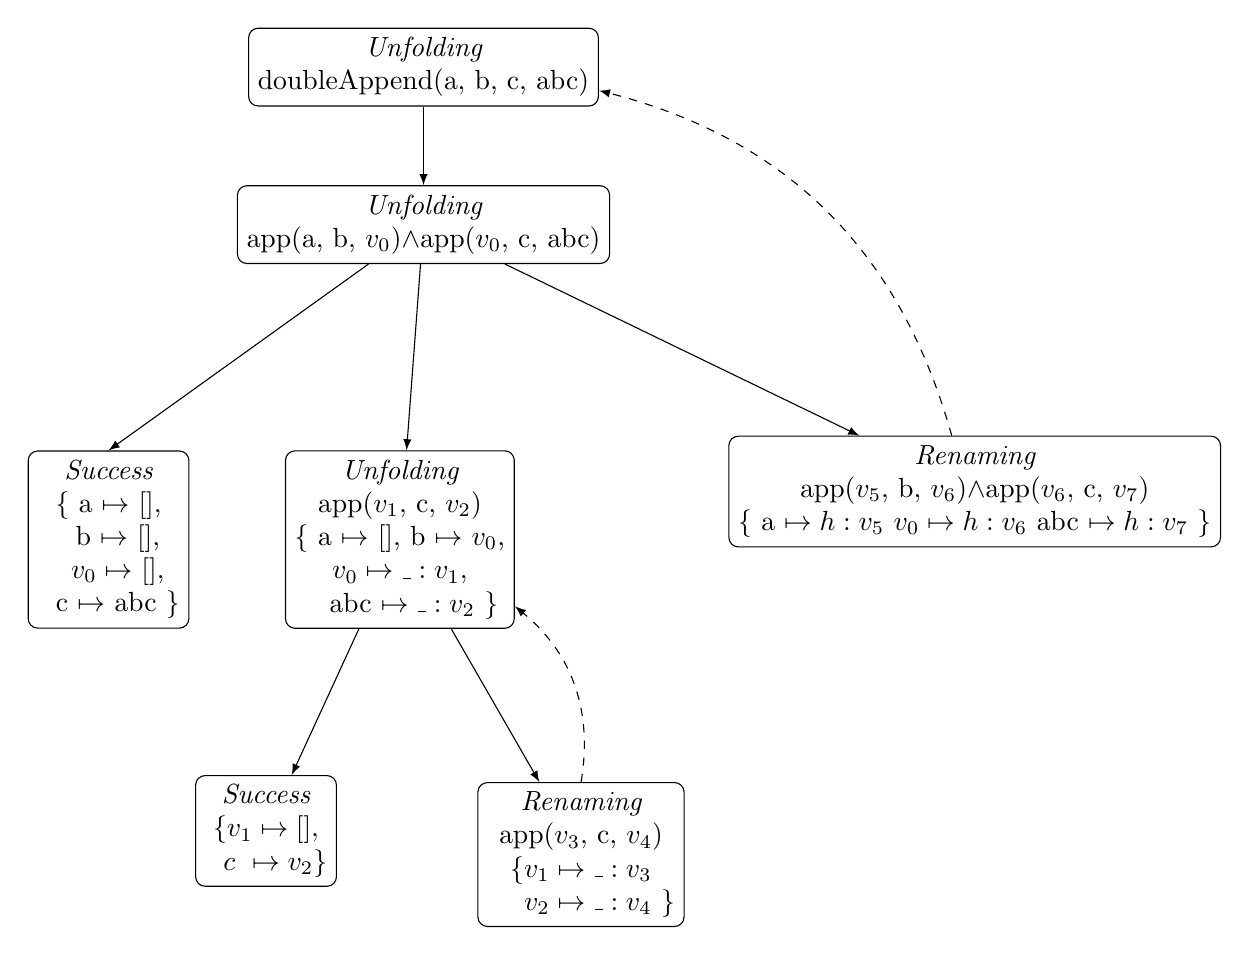
\begin{tikzpicture}[->,node distance=3cm, sibling distance=6.2cm, level distance=2cm]
  \tikzstyle{conf}=[rectangle,draw, rounded corners=.8ex,align=center]
  \node[conf] (root)   at (0, 0)     {{\it Unfolding} \\ \lstinline{doubleAppend(a, b, c, abc)}};
  \node[conf] (appapp) at (0, -2)    {{\it Unfolding} \\ \lstinline{app(a, b, $\text{v}_0$)$\land$app($\text{v}_0$, c, abc)}};
  \node[conf] (app1)   at (-0.3, -6) {{\it Unfolding} \\ \lstinline{app($\text{v}_1$, c, $\text{v}_2$)} \\ $\{$ a $\mapsto$ [], b $\mapsto$ $\text{v}_0$, \\ $\text{v}_0 \mapsto \_ : \text{v}_1$, \\ $\ \ $ abc $\mapsto \_ : \text{v}_2$ $\}$};
  \node[conf] (app2)   at (7, -5.39) {{\it Renaming} \\ \lstinline{app($\text{v}_5$, b, $\text{v}_6$)$\land$app($\text{v}_6$, c, $\text{v}_7$)} \\ $\{$ a $\mapsto \text{h} : \text{v}_5$  $\text{v}_0 \mapsto \text{h} : \text{v}_6 $  abc $\mapsto \text{h} : \text{v}_7$  $\}$};
  \node[conf] (appS)   at (-4,-6)    {{\it Success} \\ $\{$ a $\mapsto$ [], \\ \ \ b $\mapsto$ [],\\ \ \ $\text{v}_0 \mapsto$ [], \\ \ \ c $\mapsto$ abc $\}$};
  \node[conf] (app11)  at (2,  -10)  {{\it Renaming} \\ \lstinline{app($\text{v}_3$, c, $\text{v}_4$)} \\ $\{\text{v}_1 \mapsto \_ : \text{v}_3 $ \\ $\ \ \ \ \text{v}_2 \mapsto \_ : \text{v}_4 $  $\}$};
  \node[conf] (app1S)  at (-2, -9.7) {{\it Success} \\ $\{ \text{v}_1 \mapsto [],$ \\ $\ \ c \ \mapsto \text{v}_2 \}$};
  \draw[-latex] (root) -- (appapp);
  \draw[-latex] (appapp) -- (appS.north);
  \draw[-latex] (appapp) -- (app1);
  \draw[-latex] (appapp) -- (app2);
  \draw[-latex] (app1) -- (app1S);
  \draw[-latex] (app1) -- (app11);
  \draw[-latex,dashed] (app2) edge [bend right] (root);
  \draw[-latex,dashed] (app11) edge [bend right] (app1);
\end{tikzpicture}
\caption{Дерево процессов для программы \lstinline{doubleAppend}}
\label{fig:dappTree}
\end{figure}

В приведённом дереве первым этапом происходит замена определения \lstinline{doubleAppend}
на его тело. Так как в определении нет дизъюнкий, получаем всего одну конфигурацию,
в которой операцией \lstinline{fresh} добавляется новая семантическая переменная $\texttt{v}_0$.
Далее происходит обработка конфигурации с более чем одним конъюнктом. Так как используется
полная стратегия развёртывания, каждая из конъюнкий раскрывается по определению и
рассматривается их дизъюнктивная нормальная форма, в которой всего четыре дизъюнкта,
один из которых не унифицируется, поэтому всего появляется только три конфигурации.
Эти конфигурации рассматривают несколько возможных значений переменных:
\begin{enumerate}
\item когда \lstinline{a} и \lstinline{b} пустые списки, то результатом конкатенации
является \lstinline{c};
\item если же \lstinline{b} не пуст, тогда результат --- это конкатенация списков \lstinline{b} и \lstinline{c}.
      Отношение конкатенации двух списков также специализируется под задачу.
      В результате этой специализации порождается исходное отношение, поскольку
      никакой новой информации не было выявлено и исходная программа уже была оптимальна;
\item в третьем же случае выводится, что результат конкатенации трёх списков
      \lstinline{a}, \lstinline{b} и \lstinline{c} --- это конкатенация
      списков $\texttt{v}_5$, \lstinline{b} и \lstinline{c}, где $\texttt{v}_5$
      является хвостом списка, а в голову которой добавили голову \lstinline{a}.
\end{enumerate}

По данному дереву порождается остаточная программа, изображённая на рисунке~\ref{fig:dappCodeOpt}.
\begin{figure}[h!]
\begin{lstlisting}
doubleAppendo a b c d =
  fresh (x4) (app3 a b x4 c d)
app3 a b t c d =
   fresh (x7 x6 x5 x10 x9 x8)
     (a $\equiv$ [] $\land$ b $\equiv$ t $\land$
       (t $\equiv$ [] $\land$ c $\equiv$ d $\lor$
       (t $\equiv$ x8 :: x9) $\land$
        d $\equiv$ x8 :: x10 $\land$
        app2 x9 c x10
     ) $\lor$
     (a $\equiv$ x5 :: x6 $\land$
      t $\equiv$ x5 :: x7 $\land$
      d $\equiv$ x5 :: x10 $\land$
      app3 x6 b x7 c x10) ) 
app2 a b c =
  fresh (x13 x12 x11)
   (a $\equiv$ [] $\land$ b $\equiv$ c $\lor$
   (a $\equiv$ x11 :: x12 $\land$
    c $\equiv$ x11 :: x13 $\land$
    app x12 b x13))
\end{lstlisting}
\caption{Суперкомпилированная программа \lstinline{doubleAppend}}
\label{fig:dappCodeOpt}
\end{figure}

В итоге, наблюдается, как двупроходный алгоритм становится однопроходным.


\subsection{Сравнение вариаций суперкомпилятора \ukanren}

В таблицах используются условные обозначения для стратегий развёртывания:
\begin{itemize}
\item {\it Full} и {\it Full-non-rec} обозначают полную стратегию и полную стратегию развёртывания с приоритетом на нерекурсивные вызовы соответственно;
\item {\it Seq} обозначает последовательную стратегию развёртывания;
\item {\it Non-rec} и {\it Rec} обозначают нерекурсивную и рекурсивную стратегии соответственно;
\item {\it Min} и {\it Max} обозначают минимальную и максимальную стратегии соответственно;
\item {\it First} обозначает стратегию, при которой всегда развёртывается первый конъюнкт.
\end{itemize}

А также для суперкомпиляторов:
\begin{itemize}
\item {\it Б.С.} обозначает базовый суперкомпилятор с обобщением вниз на предков;
\item {\it М.1 } обозначает модификацию, при которой происходит запрет на обобщение после обобщения;
\item {\it M.2 } обозначает модификацию, при которой обобщение происходит на все вычисленные вершины;
\item {\it M.3 } обозначает модификацию, при которой происходит обобщение вверх на родительские вершины;
\item {\it M.4 } обозначает модификацию, при которой происходит обобщение вверх на родительские вершины, кроме корневой.

\end{itemize}


В таблице~\ref{fig:dappTest} представлены результаты сравнения модификаций
с базовым суперкомпилятором при разных стратегиях развёртывания.
При полных стратегиях для \lstinline{doubleAppendo} возникает эффект дефорестации.
В остальных стратегиях этого не происходит, из-за чего исполнения по
крайней мере в два раза хуже. Из-за того, что программа довольно небольшая,
модификации алгоритма суперкомпиляции хотя не и оказывают влияния, результат не портят.

\begin{table}[h!]
\center
\begin{tabular}{|l|c|c|c|c|c|}
\hline
                   &{\it Б.С.}&{\it М.1}&{\it М.2}&{\it М.3}&{\it M.4} \\ \hline
{\it Full        } &{\bf 0.0040}  & {\bf 0.0040 } & {\bf 0.0041 } & {\bf 0.0042 } & {\bf 0.0040 }  \\ \hline
{\it Full-non-rec} &{\bf 0.0039}  & {\bf 0.0040 } & {\bf 0.0037 } & {\bf 0.0039 } & {\bf 0.0040 }  \\ \hline
{\it Seq         } &0.0094  &  0.0099 & 0.0093 &0.0096 & 0.0127  \\ \hline
{\it Non-rec     } &0.0100  &  0.0097 & 0.0096 &0.0097 & 0.0097  \\ \hline
{\it Rec         } &0.0096  &  0.0096 & 0.0094 &0.0099 & 0.0092  \\ \hline
{\it Min         } &0.0097  &  0.0097 & 0.0103 &0.0095 & 0.0096  \\ \hline
{\it Max         } &0.0095  &  0.0110 & 0.0096 &0.0094 & 0.0094  \\ \hline
{\it First       } &0.0099  &  0.0095 & 0.0096 &0.0092 & 0.0098  \\ \hline
\end{tabular}
\caption{Результат для \lstinline{doubleAppendo} c конкатенацией трёх списков длины 120, секунды}
\label{fig:dappTest}
\end{table}

В таблице~\ref{fig:maxlenTest} указаны результаты тестирования для
программы \lstinline{maxLengtho}.

\begin{table}[h!]
\center
\begin{tabular}{|l|c|c|c|c|c|}
\hline
                  &{\it Б.С.}   &{\it М.1}      &{\it М.2}      &{\it М.3}&{\it M.4} \\ \hline
{\it Full        }& 0.614       & 0.634        & {\bf 0.249}  & {\bf 0.254} & {\bf 0.252} \\ \hline
{\it Full-non-rec}& 0.611       & 0.607        & 0.594        & {\bf 0.252} & {\bf 0.246} \\ \hline
{\it Seq         }& {\bf 0.279} & {\bf 0.281}  & 0.280        & 0.279  & 0.280 \\ \hline
{\it Non-rec     }& {\bf 0.276} & {\bf 0.281}  & 0.277        & 0.275  & 0.281 \\ \hline
{\it Rec         }& 0.857       & 0.867        & 0.560        & 0.562  & 0.560 \\ \hline
{\it Min         }& {\bf 0.280} & 0.283        & 0.288        & 0.282  & 0.280 \\ \hline
{\it Max         }& {\bf 0.286} & 0.282        & 0.279        & 0.281  & 0.277 \\ \hline
{\it First       }& 0.861       & 0.868        & 0.564        & 0.948  & 0.950 \\ \hline


\end{tabular}
\caption{Запуск для \lstinline{maxLengtho} на списке \lstinline{[1..200]}, секунды}
\label{fig:maxlenTest}
\end{table}

В таблице~\ref{fig:sortTest} указаны результаты тестирования для
программы \lstinline{sorto}.

\begin{table}[h!]

\center
\begin{tabular}{|l|c|c|c|c|c|}
\hline
                  &{\it Б.С.}&{\it М.1}&{\it М.2}&{\it М.3}&{\it M.4} \\ \hline
{\it Full        }&0.260       & 0.259        &  0.263       & 0.258       & {\bf 0.251} \\ \hline
{\it Full-non-rec}&0.255       & {\bf 0.250}  &  0.259       & 0.258       & {\bf 0.252} \\ \hline
{\it Seq         }&{\bf 0.254} & {\bf 0.250}  &  {\bf 0.252} & {\bf 0.251} & 0.264 \\ \hline
{\it Non-rec     }&0.256       & 0.262        &  0.260       & 0.255       & 0.263 \\ \hline
{\it Rec         }&0.261       & 0.259        &  0.263       & 0.266       & 0.268 \\ \hline
{\it Min         }&0.260       & 0.261        &  0.265       & 0.272       & 0.261 \\ \hline
{\it Max         }&0.268       & 0.257        &  0.273       & {\bf 0.251} & 0.257 \\ \hline
{\it First       }&0.255       & 0.261        &  0.263       & 0.256       & 0.260 \\ \hline
\end{tabular}
\caption{Запуск для \lstinline{sort}}
\label{fig:sortTest}
\end{table}

В таблице~\ref{fig:sortTest} указаны результаты тестирования для
программы \lstinline{loginto}, которая использовалась для генерации всех выполнимых формул
без свободных переменных.

\begin{table}[h!]
\center
\begin{tabular}{|l|c|c|c|c|c|}
\hline
   &{\it Б.С.}&{\it М.1}&{\it М.2}&{\it М.3}&{\it M.4} \\ \hline
{\it Full        } &    -        &    -         & 0.1318       &  0.1049       &    -   \\ \hline
{\it Full-non-rec} & {\bf 0.076} & 0.0716       & 0.2097       &  0.1115       & 0.1258 \\ \hline
{\it Seq         } & 0.168       & 0.1811       & 0.1491       &  0.0902       & {\bf 0.0913} \\ \hline
{\it Non-rec     } & 0.078       & 0.0921       & 0.1356       &  0.0883       & 0.1144 \\ \hline
{\it Rec         } & 0.081       & 0.0740       & {\bf 0.0954} &  {\bf 0.0637} & 0.1263 \\ \hline
{\it Min         } & 0.080       & {\bf 0.0639} & 0.1097       &  0.0921       & 0.1170 \\ \hline
{\it Max         } & 0.164       & 0.1929       & 0.1438       &  0.0775       & 0.1108 \\ \hline
{\it First       } & 0.181       & 0.1636       & 0.1757       &  0.0701       & 0.1894 \\ \hline
\end{tabular}
\caption{Запуск для loginto \todo{subst0}}
\end{table}

\begin{table}[h!]
\center
\begin{tabular}{|l|c|c|c|c|c|}
\hline
   &{\it Б.С.}&{\it М.1}&{\it М.2}&{\it М.3}&{\it M.4} \\ \hline
{\it Full        }&    -         &     -        & 0.078       & 0.068 &    -  \\ \hline
{\it Full-non-rec}& 0.056        &  0.045       & 0.125       & 0.084 & 0.082 \\ \hline
{\it Seq         }& 0.109        &  0.110       & 0.086       & 0.063 & 0.074 \\ \hline
{\it Non-rec     }& {\bf 0.046}  &  {\bf 0.038} & 0.081       & 0.072 & {\bf 0.067} \\ \hline
{\it Rec         }& 0.055        &  0.050       & 0.074       & {\bf 0.055} & 0.079 \\ \hline
{\it Min         }& 0.053        &  0.041       & {\bf 0.066} & {\bf 0.055} & 0.079 \\ \hline
{\it Max         }& 0.100        &  0.117       & 0.108       & 0.057 & 0.074 \\ \hline
{\it First       }& 0.118        &  0.103       & 0.091       & 0.068 & 0.101 \\ \hline
\end{tabular}
\caption{Запуск для loginto \todo{subst1}}
\end{table}

\begin{table}[h!]
\center
\begin{tabular}{|l|c|c|c|c|c|}
\hline
   &{\it Б.С.}&{\it М.1}&{\it М.2}&{\it М.3}&{\it M.4} \\ \hline
{\it Full        }&    -        &    -        & 0.078       & 0.062      &    - \\ \hline
{\it Full-non-rec}& 0.137       & 0.040       & 0.093       & 0.042      & 0.069 \\ \hline
{\it Seq         }& 0.086       & 0.082       & 0.066       & 0.049      & {\bf 0.050} \\ \hline
{\it Non-rec     }& 0.043       & {\bf 0.031} & 0.063       & 0.044      & 0.055 \\ \hline
{\it Rec         }& {\bf 0.037} & 0.034       & {\bf 0.045} & 0.040      & 0.051 \\ \hline
{\it Min         }& {\bf 0.037} & 0.039       & 0.049       & 0.041      & 0.054 \\ \hline
{\it Max         }& 0.068       & 0.070       & 0.067       &{\bf 0.036} & 0.062 \\ \hline
{\it First       }& 0.104       & 0.100       & 0.110       & 0.095      & 0.137 \\ \hline
\end{tabular}
\caption{Запуск для loginto \todo{subst1}}
\end{table}


Несмотря на то, что разные подходы на разных классах программ показывают
себя с лучшей стороны, в среднем модификация с обобщением вверх показывает себя
лучше всего.


\subsection{Сравнение суперкомпилятора с существующими решениями}

В таблице~\ref{fig:totalResult}

\begin{table}[h!]
\center
\begin{tabular}{|c|c|c|c|c|c|}
\hline
{\it Параметр} & {\it Оригинал} & {\it ECCE }  & {\it CPD} & {\bf Б.C} & {\bf N.R.M.3} \\ \hline
{\bf doubleAppend} & \multicolumn{5}{|l|}{списки длины 120 } \\ \hline
                   & 0.0135 & 0.0051 & 0.0133 & {\bf 0.0040} & 0.0097 \\ \hline


{\bf maxLength} & \multicolumn{5}{|l|}{список [1..200]} \\ \hline

                & 0.257 & {\bf 0.230} & 0.727 & 0.614 & 0.275 \\ \hline


%\rowcolor{black!10}
{\bf sort} & \multicolumn{5}{|l|}{случайный список длины 50 } \\ \hline
         & 8.42     & 12.28 & 13.2 & 0.28  & {\bf 0.25} \\ \hline

%\rowcolor{black!10}
% {\bf isPath} & \multicolumn{4}{|l|}{произвольный путь длины 10} \\ \hline
% граф 1 & > 300    & 9     & 10   & 0.25   \\ 
% граф 2 &          & 2.7   & 2.8  & 0.1    \\
% % граф 3 &          & 0.35  & 0.4  & 0.006  \\
% \hline

%\rowcolor{black!10}
{\bf logint} & \multicolumn{5}{|l|}{размер подстановки} \\ \hline
0 & > 300    & 0.17  & 2.7  & -  &  {\bf 0.08} \\
1 &          & 0.09  & 1.7  & -  &  {\bf 0.07} \\
2 &          & 0.08   & 0.9  & -  & {\bf 0.04} \\
\hline

%\rowcolor{black!10}
%{\bf lam} & \multicolumn{4}{|l|}{редуцируются} \\ \hline
%10 термов к себе    & 0.17     & 0.001 & 0.008 & 0.002  \\
%50 термов к себе    & > 300    & 2.98  & 4.32  & 1.89   \\
%1000 термов к const & 1.01     & 0.126 & 0.263 & 0.274  \\
%\hline
\end{tabular}
\caption{Тестовые результаты, cекунды}
\label{fig:totalResult}
\end{table}


